%%%%%%%%%%%%%%%%%%%%%%%%%%%%%%%%%%%%%%%%%
% Masters/Doctoral Thesis 
% LaTeX Template
% Version 2.5 (27/8/17)
%
% This template was downloaded from:
% http://www.LaTeXTemplates.com
%
% Version 2.x major modifications by:
% Vel (vel@latextemplates.com)
%
% This template is based on a template by:
% Steve Gunn (http://users.ecs.soton.ac.uk/srg/softwaretools/document/templates/)
% Sunil Patel (http://www.sunilpatel.co.uk/thesis-template/)
%
% Template license:
% CC BY-NC-SA 3.0 (http://creativecommons.org/licenses/by-nc-sa/3.0/)
%
%%%%%%%%%%%%%%%%%%%%%%%%%%%%%%%%%%%%%%%%%

%----------------------------------------------------------------------------------------
%	PACKAGES AND OTHER DOCUMENT CONFIGURATIONS
%----------------------------------------------------------------------------------------

\documentclass[
11pt, % The default document font size, options: 10pt, 11pt, 12pt
%oneside, % Two side (alternating margins) for binding by default, uncomment to switch to one side
english, % ngerman for German
singlespacing, % Single line spacing, alternatives: onehalfspacing or doublespacing
%draft, % Uncomment to enable draft mode (no pictures, no links, overfull hboxes indicated)
%nolistspacing, % If the document is onehalfspacing or doublespacing, uncomment this to set spacing in lists to single
%liststotoc, % Uncomment to add the list of figures/tables/etc to the table of contents
%toctotoc, % Uncomment to add the main table of contents to the table of contents
%parskip, % Uncomment to add space between paragraphs
%nohyperref, % Uncomment to not load the hyperref package
headsepline, % Uncomment to get a line under the header
%chapterinoneline, % Uncomment to place the chapter title next to the number on one line
%consistentlayout, % Uncomment to change the layout of the declaration, abstract and acknowledgements pages to match the default layout
]{MastersDoctoralThesis} % The class file specifying the document structure

\usepackage[utf8]{inputenc} % Required for inputting international characters
\usepackage[T1]{fontenc} % Output font encoding for international characters
\usepackage{physics}
\usepackage[caption=false]{subfig}



%\usepackage{mathpazo} % Use the Palatino font by default

\usepackage[backend=biber,style=ieee,natbib=true]{biblatex} % Use the bibtex backend with the authoryear citation style (which resembles APA)

\addbibresource{example.bib} % The filename of the bibliography

\usepackage[autostyle=true]{csquotes} % Required to generate language-dependent quotes in the bibliography

%----------------------------------------------------------------------------------------
%	MARGIN SETTINGS
%----------------------------------------------------------------------------------------

\geometry{
	paper=a4paper, % Change to letterpaper for US letter
	inner=2.5cm, % Inner margin
	outer=3.8cm, % Outer margin
	bindingoffset=.5cm, % Binding offset
	top=1.5cm, % Top margin
	bottom=1.5cm, % Bottom margin
	%showframe, % Uncomment to show how the type block is set on the page
}

%----------------------------------------------------------------------------------------
%	THESIS INFORMATION
%----------------------------------------------------------------------------------------

\thesistitle{Automatic Pattern Recognition in Solids based on Machine Learning} % Your thesis title, this is used in the title and abstract, print it elsewhere with \ttitle
\supervisor{Prof. Dr. Stefan \textsc{Goedecker}} % Your supervisor's name, this is used in the title page, print it elsewhere with \supname
\examiner{} % Your examiner's name, this is not currently used anywhere in the template, print it elsewhere with \examname
\degree{ } % Your degree name, this is used in the title page and abstract, print it elsewhere with \degreename
\author{Matthias \textsc{Vogler}} % Your name, this is used in the title page and abstract, print it elsewhere with \authorname
\addresses{} % Your address, this is not currently used anywhere in the template, print it elsewhere with \addressname

\subject{Computational Physics} % Your subject area, this is not currently used anywhere in the template, print it elsewhere with \subjectname
\keywords{} % Keywords for your thesis, this is not currently used anywhere in the template, print it elsewhere with \keywordnames
\university{{University of Basel}} % Your university's name and URL, this is used in the title page and abstract, print it elsewhere with \univname
\department{{Departement of Physics}} % Your department's name and URL, this is used in the title page and abstract, print it elsewhere with \deptname
\group{{Computational Physics}} % Your research group's name and URL, this is used in the title page, print it elsewhere with \groupname
\faculty{{Faculty of Science}} % Your faculty's name and URL, this is used in the title page and abstract, print it elsewhere with \facname

\AtBeginDocument{
\hypersetup{pdftitle=\ttitle} % Set the PDF's title to your title
\hypersetup{pdfauthor=\authorname} % Set the PDF's author to your name
\hypersetup{pdfkeywords=\keywordnames}
\hypersetup{colorlinks=false} % Set the PDF's keywords to your keywords
}


\begin{document}

\frontmatter % Use roman page numbering style (i, ii, iii, iv...) for the pre-content pages

\pagestyle{plain} % Default to the plain heading style until the thesis style is called for the body content

%----------------------------------------------------------------------------------------
%	TITLE PAGE
%----------------------------------------------------------------------------------------

\begin{titlepage}
\begin{center}

\vspace*{.06\textheight}
{\scshape\LARGE \univname\par}\vspace{1.5cm} % University name
\textsc{\Large Project Thesis}\\[0.5cm] % Thesis type

\HRule \\[0.4cm] % Horizontal line
{\huge \bfseries \ttitle\par}\vspace{0.4cm} % Thesis title
\HRule \\[1.5cm] % Horizontal line
 
\begin{minipage}[t]{0.4\textwidth}
\begin{flushleft} \large
\emph{Author:}\\
{\authorname} % Author name - remove the \href bracket to remove the link
\end{flushleft}
\end{minipage}
\begin{minipage}[t]{0.4\textwidth}
\begin{flushright} \large
\emph{Supervisor:} \\
{\supname} % Supervisor name - remove the \href bracket to remove the link  
\end{flushright}
\end{minipage}\\[3cm]
 
\vfill

\deptname\\[2cm] % Research group name and department name
 
\vfill

{\large \today}\\[4cm] % Date
%\includegraphics{Logo} % University/department logo - uncomment to place it
 
\vfill
\end{center}
\end{titlepage}

%----------------------------------------------------------------------------------------
%	DECLARATION PAGE
%----------------------------------------------------------------------------------------

\begin{declaration}
\addchaptertocentry{\authorshipname} % Add the declaration to the table of contents
\noindent I, \authorname, declare that this thesis titled, \enquote{\ttitle} and the work presented in it are my own. I confirm that:

\begin{itemize} 
\item This work was done wholly or mainly while in candidature for a research degree at this University.
\item Where any part of this thesis has previously been submitted for a degree or any other qualification at this University or any other institution, this has been clearly stated.
\item Where I have consulted the published work of others, this is always clearly attributed.
\item Where I have quoted from the work of others, the source is always given. With the exception of such quotations, this thesis is entirely my own work.
\item I have acknowledged all main sources of help.
\item Where the thesis is based on work done by myself jointly with others, I have made clear exactly what was done by others and what I have contributed myself.\\
\end{itemize}
 
\noindent Signed:\\
\rule[0.5em]{25em}{0.5pt} % This prints a line for the signature
 
\noindent Date:\\
\rule[0.5em]{25em}{0.5pt} % This prints a line to write the date
\end{declaration}

\cleardoublepage

%----------------------------------------------------------------------------------------
%	QUOTATION PAGE
%----------------------------------------------------------------------------------------



%----------------------------------------------------------------------------------------
%	ABSTRACT PAGE
%----------------------------------------------------------------------------------------

\begin{abstract}
\addchaptertocentry{\abstractname} % Add the abstract to the table of contents
The Thesis Abstract is written here (and usually kept to just this page). The page is kept centered vertically so can expand into the blank space above the title too\ldots
\end{abstract}

%----------------------------------------------------------------------------------------
%	ACKNOWLEDGEMENTS
%----------------------------------------------------------------------------------------

\begin{acknowledgements}
\addchaptertocentry{\acknowledgementname} % Add the acknowledgements to the table of contents
The acknowledgments and the people to thank go here, don't forget to include your project advisor\ldots
\end{acknowledgements}

%----------------------------------------------------------------------------------------
%	LIST OF CONTENTS/FIGURES/TABLES PAGES
%----------------------------------------------------------------------------------------

\tableofcontents % Prints the main table of contents

\listoffigures % Prints the list of figures

\listoftables % Prints the list of tables

%----------------------------------------------------------------------------------------
%	ABBREVIATIONS
%----------------------------------------------------------------------------------------

% \begin{abbreviations}{ll} % Include a list of abbreviations (a table of two columns)

% \textbf{LAH} & \textbf{L}ist \textbf{A}bbreviations \textbf{H}ere\\
% \textbf{WSF} & \textbf{W}hat (it) \textbf{S}tands \textbf{F}or\\

% \end{abbreviations}

%----------------------------------------------------------------------------------------
%	PHYSICAL CONSTANTS/OTHER DEFINITIONS
%----------------------------------------------------------------------------------------

% \begin{constants}{lr@{${}={}$}l} % The list of physical constants is a three column table

% % The \SI{}{} command is provided by the siunitx package, see its documentation for instructions on how to use it

% Speed of Light & $c_{0}$ & \SI{2.99792458e8}{\meter\per\second} (exact)\\
% %Constant Name & $Symbol$ & $Constant Value$ with units\\

% \end{constants}

%----------------------------------------------------------------------------------------
%	SYMBOLS
%----------------------------------------------------------------------------------------

% \begin{symbols}{lll} % Include a list of Symbols (a three column table)

% $a$ & distance & \si{\meter} \\
% $P$ & power & \si{\watt} (\si{\joule\per\second}) \\
% %Symbol & Name & Unit \\

% \addlinespace % Gap to separate the Roman symbols from the Greek

% $\omega$ & angular frequency & \si{\radian} \\

% \end{symbols}

%----------------------------------------------------------------------------------------
%	DEDICATION
%----------------------------------------------------------------------------------------


%----------------------------------------------------------------------------------------
%	THESIS CONTENT - CHAPTERS
%----------------------------------------------------------------------------------------

\mainmatter % Begin numeric (1,2,3...) page numbering

\pagestyle{thesis} % Return the page headers back to the "thesis" style

% Include the chapters of the thesis as separate files from the Chapters folder
% Uncomment the lines as you write the chapters

% Chapter 1

\chapter{Theory} % Main chapter title

\label{Chapter1} % For referencing the chapter elsewhere, use \ref{Chapter1} 

%----------------------------------------------------------------------------------------

% Define some commands to keep the formatting separated from the content 
\newcommand{\keyword}[1]{\textbf{#1}}
\newcommand{\tabhead}[1]{\textbf{#1}}
\newcommand{\code}[1]{\texttt{#1}}
\newcommand{\file}[1]{\texttt{\bfseries#1}}
\newcommand{\option}[1]{\texttt{\itshape#1}}

%----------------------------------------------------------------------------------------

\section{Atomar Fingerprints}
Atomar fingerprints can be used to measure similiarities and dissimilarities between different molecular structures and the atoms within. Quantizing the similarity between two structures just from measurement data is not a straight forward process, since the data only holds the cartesian coordinates of the atoms within the cell and the lattice vectors of said cell. These  quantities are not directly suitable for distinguishing different structures or the atoms within. The reasons are that the translation vectors are not unique and maybe transformed into linear combinations of themselves and still describe the same structure. Furthermore, the coordinates and cell parameters can contain numerical noise and all the positions of the atoms maybe translated by an arbitrary vector as described by \citeauthor{Lonie2012} \cite{Lonie2012}. A fingerprint is then an abstract measure of characteristic for a structure that can be based on the afformentioned quantities but has the property of being easily comparable to other structures to test their similarity. The fingerprint discussed in this work is the one proposed by \citeauthor{Zhu2016} \cite{Zhu2016}. The environemnt of each atom is described by a fingerprint vector. This fingerprint vector can be calculated out of the experimental data which includes the position of the atoms in the structure in cartesian coordinates and the lattice vectors of the structure. \\
\section{Calculation of the Fingerprint}
For each atom $k$ located at $\mathbf{R}_k$ in the crystal, we consider all neighbouring atoms contained in a sphere around $\mathbf{R}_k$. On each of those atoms, we put one or more Gaussian type orbitals, and calculate an overlap matrix as described by \citeauthor{Sadeghi2013} \cite{Sadeghi2013}.
\subsection{Overlap Matrix}
The overlap matrix of the Gaussian type Orbitals (GTO) has similar properties as the Hamiltonian but is easily calculated analytically according to \citeauthor{Sadeghi2013} \cite{Sadeghi2013}. For this they introduce the normalized GTO's centered at the atomic positions $\mathbf{r}_i$ as
\begin{equation}\phi_i^l(\mathbf{r})=N_l(x-x_i)^{l_x}(y-y_j)^{l_y}(z-z_i)^{l_z}e^{-\alpha_i||\mathbf{r}-\mathbf{r}_i||^2}.\end{equation}
With $L=l_x+l_y+l_z$ as the angular momentum. The Gaussian width $\alpha_i$ is proportional to the inverse of the covalent radius of atom $i$. In our work we modified the Gaussian width $\alpha_i$ further to depend on the orbital eigenenergy of the corresponding orbitals. The orbitals considered were the 2s and 2p orbitals of Nitrogen and Carbon. The dependence on these energies was defined as:
\begin{equation}\label{eq:const}\tilde{\alpha}_i=C\cdot\frac{\alpha_i}{\left|E_{Orbital}\right|}.\end{equation} 
The constant $C$ was then experimentaly determined. In the remainder of this work we will omit the tilde of $\tilde{\alpha}_i$.\\
The overlap integral of two GTO's is
\begin{equation}\left<\phi_i^l\right|\left.\phi_j^{l'}\right>=\int d\mathbf{r}\,\phi_i^l(\mathbf{r})\phi^{l'}_j(\mathbf{r})\end{equation}
and gives the normalization factors as
\begin{equation}N_l(\alpha_i)=\frac{1}{\sqrt{\left<\phi_i^l\right|\left.\phi_i^l\right>}}=\left(\frac{2\alpha_i}{\pi}\right)^{\frac{3}{4}}\sqrt{n_{l_x}n_{l_y}n_{l_z}},\end{equation}
with
$$n_k=\frac{(4\alpha_i)^k}{(2k-1)!!}.$$
The Orbitals are then obtained by differentiating
$$\phi_i^s(\mathbf{r})=\left(\frac{2\alpha_i}{\pi}\right)^{\frac{3}{4}}e^{-\alpha_i||\mathbf{r}-\mathbf{r}_i||^2}$$
as
\begin{equation}\phi_i^{p_j}=\frac{1}{\sqrt{\alpha_i}}\frac{\partial\phi_i^s(\mathbf{r})}{\partial r_j}.\end{equation}
The simplified relation for calculating the elements of the overlap matrix according to \citeauthor{Clementi1966} \cite{Clementi1966} are then
\begin{equation}
\label{ovrlap}
S_{ij}=S_{ji}=\left(\frac{2\sqrt{\alpha_i\alpha_j}}{\alpha_i+\alpha_j}\right)^\frac{3}{2}\exp\left[\frac{-\alpha_i\alpha_j}{\alpha_i+\alpha_j}r_{ij}^2\right],\end{equation}
for the $s$-$s$ overlap. The $s$-$p$ overlap and the $p$-$p$ overlap are then obtained by
\begin{equation}
\begin{aligned}
\bra{\phi_i^{p_x}}\ket{\phi_j^s} &= \frac{1}{\sqrt{\alpha_i}}\frac{\partial S_{ij}}{\partial x_i}=-\left(\frac{2\sqrt{\alpha_i}\alpha_j}{\alpha_i+\alpha_j}\right)(x_i-x_j)S_{ij} \\
\bra{\phi_i^{p_x}}\ket{\phi_j^{p_{x'}}}&=\left(\frac{2\sqrt{\alpha_i\alpha_j}}{\alpha_i+\alpha_j}\right)S_{ij}\left[\delta_{x,x'}-\frac{2\alpha_i\alpha_j}{\alpha_i+\alpha_j}(x_i-x_j)(x'_i-x'_j)\right].
\end{aligned}
\end{equation}

\subsection{Amplitude weighing}
The overlap matrix $S^k_{ij}$ for the $k$-th atom in the sphere is now defined as
\begin{equation}S^k_{ij}=\int d\mathbf{r}\, G_i(\mathbf{r}-\mathbf{R}_{w(i)})G_j(\mathbf{r}-\mathbf{R}_{w(j)})\end{equation}
where the Gaussians are normalized to one and the width of each Gaussian $G_i(\mathbf{r})$ is given by the covalent radius of the atom $w(i)$ as in \cite{Zhu2016} and the eigenenergy of the respective orbital. At the sphere boundaries there might be discontinuities in the eigenvalues when atoms enter or leave the sphere. For that reason one constructs a matrix $T^k$ such that
\begin{equation}T^k_{ij}=f_c(|\mathbf{R}_{w(i)}-\mathbf{R}_k)S^k_{ij}f_c(\mathbf{R}_{w(j)}-\mathbf{R}_k)),\end{equation}
with $f_c$ a cuttoff function which goes smoothly to zero on the surface of the sphere
\begin{equation}f_c(r)=\left(1-\frac{r^2}{2n\sigma_c^2}\right)^n.\end{equation}
The eigenvalues of $T^k$ sorted in descending orders form the fingerprint of the atomic environement of the atom $k$. The number of entries in this fingerprint vector depend on the number of atoms in the sphere. Since this number can be different for each configuration, one assumes a maximum length for the vector. Subsequent entries that are not touched on by the fingerprint, are just set to zero \cite{Zhu2016}.
\subsection{Measuring similarity}
The euclidian distance between two fingerprint vectors $\mathbf{V}_i$, $\mathbf{V}_j$ 
\begin{equation}\label{fp_dist}
d_{i,j}=|\mathbf{V}_i-\mathbf{V}_j|
\end{equation}
is now a direct measure for the similarity of two atomic environments. This can be expanded to measuring similarities between crystals themselves. The atomic fingerprints $\mathbf{V}_p^k$ and $\mathbf{V}_k^q$ of all the $N_{at}$ atoms in two configurations $p$ and $q$ can be used to calculate a configurational disctance $d(p,q)$ between the two crystals \cite{Zhu2016}
\begin{equation}d(p,q)=\text{min}_p\left(\sum_k^{N_{at}}|\mathbf{V}^p_k-\mathbf{V}^q_{P(k)}|^2\right)^{\frac{1}{2}}.\end{equation}
$P$ is a permutation which matches atoms in crystal $p$ to atoms in crystal $q$. The permutation which minimizes $d(p,q)$ can be found via the Hungarian algorithm \cite{Kuhn1955}. However for this work, we are mainly interested in the atomic environments and not in the fingerprints for clusters.
\newpage
\section{Maximum Volume Simplex Method}
The method of the maximum volume simplex was proposed by \citeauthor{Behnam2020} \cite{Behnam2020} and gives a way to do the inverse operation to calculating fingerprint distances. It calculates the fingerprint vectors from a given set of fingerprint distances. These fingerprints are the corners of a simplex or particularly the largest volume simplex. The corners of this largest volume simplex correspond to landmark environements, which then in turn can be used to classify fingerprints compared to the corners. This gives us a method of \emph{training} a simplex on a set of fingerprints and their configurations and then evaluating its result on a test set of configurations. In the following sections we will give a brief review of the largest volume simplex method as it was described in the original paper \cite{Behnam2020}.
\subsection{Obtaining fingerprint vectors from fingerprint distances}
Given a set of pairwise fingerprint distances $d_{ij}$, see eq. (\ref{fp_dist}), we want to find a set of points $\mathbf{x}^i$ which satisfy the constraint
\begin{equation}d_{ij}=|\mathbf{x}^i-\mathbf{x}^j|.\end{equation}
Requiring that the first point $\mathbf{x}^0$ is at the origin and that for each consecutive point the number of nonzero components increases by one makes the solution to the problem unique. The points $\mathbf{x}^i$ have the following structure:
\begin{equation} (\mathbf{x}^1, \mathbf{x}^2, \ldots, \mathbf{x}^N) = 
\left(\begin{matrix}
x_{1,1} & x_{1,2} & \cdots & x_{1,N} \\
0 & x_{2,2} &\cdots & x_{2,N} \\
\vdots & \vdots & \ddots & \vdots \\
0 & 0 & 0 & x_{N,N}   
\end{matrix}\right)
\end{equation}
With the first point at the origin, the next point is placed on the positive x-axis at the corresponding distance with the 3rd point on the xy-plane and so on. We can then aquire the components of the points $\mathbf{x}^i$ with simple relations recursivly from the distances $d_{ij}$. The distance of $\mathbf{x}^N$ to the origin $\mathbf{x}^0$ is given by its norm
\begin{equation}d_{0,N}^2=\sum_{i=1}^N x_{i,N}^2.\end{equation}
The difference between column $N$ and $M$ for $M<N$ is related to the distance of $\mathbf{x}^N$ and $\mathbf{x}^M$ as
\begin{equation}\label{eq:1}
 d^2_{M,N}=\sum_{i=1}^M(x_{i,N}-x_{i,M})^2+\sum_{j=M+1}^N x^2_{j,N}.\end{equation}

Now one can take the difference between $d^2_{M,N}$ and $d^2_{0,N}$ and obtain a set of equations
\begin{equation}d^2_{M,N}-d^2_{0,N}=\sum_{i=1}^M -x_{i,M}(2x_{i,N} - x_{i,M}).\end{equation}
Out of (\ref{eq:1}) one can extract a general relation for $M<N$:
\begin{equation}
x_{M,N}=\frac{d^2_{0,M}+d^2_{0,N}-d^2_{M,N}-2\sum_{i=1}^{M-1} x_{i,M} x_{i,N} } {2x_{M,M}}
\end{equation}
For $M=N$ we get:
\begin{equation}
x_{M,N}=\sqrt{d^2_{0,N}-\sum_{i=1}^{N-1}x^2_{i,N}}
\end{equation}
The points $\mathbf{x}^i$ are now our fingerprint vectors extracted from the distances $d_{ij}$. 
\subsection{Constructing the largest volume simplex}
Constructing the largest simplex is done by first identifying the two environements with largest distance. These define the origin $\mathbf{x}^0$ and the first point on the x-axis $\mathbf{x}^1$. Our simplex at this stage ist just a line. The next step is to identify the environment which will give the largest area triangle with the point $\mathbf{x}^2$. This procedure is then repeated and corners are added to the simplex until adding a subsequent corner at step $l$ would collapse the total volume, meaning that further fingerprints are quasi linearly dependent on the previous ones. This procedure identifies from our \emph{trainings set} the landmark configurations, to which we can compare our \emph{test configurations}.
% Chapter Template

\chapter{Implementation and Results} % Main chapter title

\label{Chapter2} % Change X to a consecutive number; for referencing this chapter elsewhere, use \ref{ChapterX}

%----------------------------------------------------------------------------------------
%	SECTION 1
%----------------------------------------------------------------------------------------

\section{Implementation}
The code base worked with, was a direct Fortran90 implementation of the fingerprint algorithm proposed by \cite{Zhu2016}. The compiler used for all computation was the GNU Fortran compiler \cite{gnufortran}.

\subsection{Data}
The structures used for evaluating our methods were carbon-nitrate crystals. The data contained the positions of the atoms in cartesian coordinates and the lattice vectors of the unit cell. We thank Prof. Alireza Ghasemi for providing us with the data base of carbon-nitate structures that we have analysed.


\begin{figure}[p]
\center
\label{fig:structures}
\subfloat[8 atom unit cell]{%
  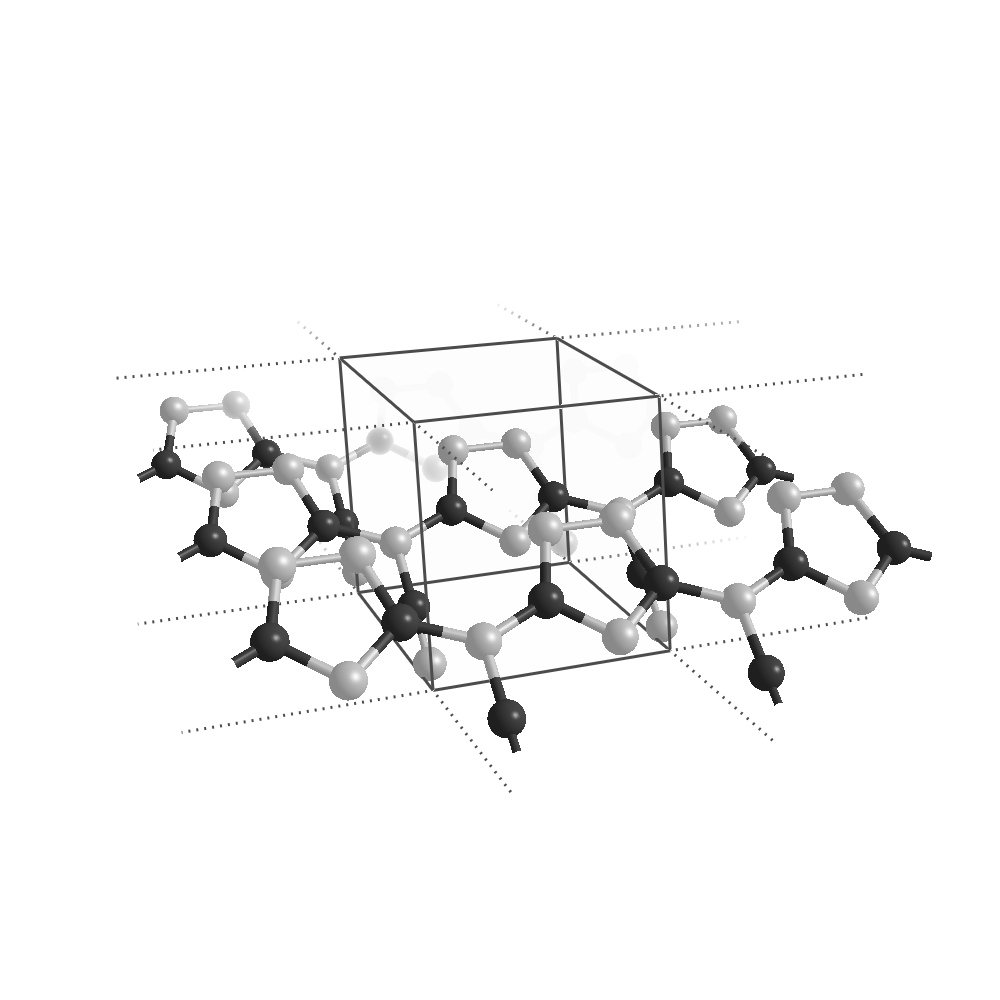
\includegraphics[clip,scale=0.3]{Figures/8structure.png}%
}

\subfloat[16 atom unit cell]{%
  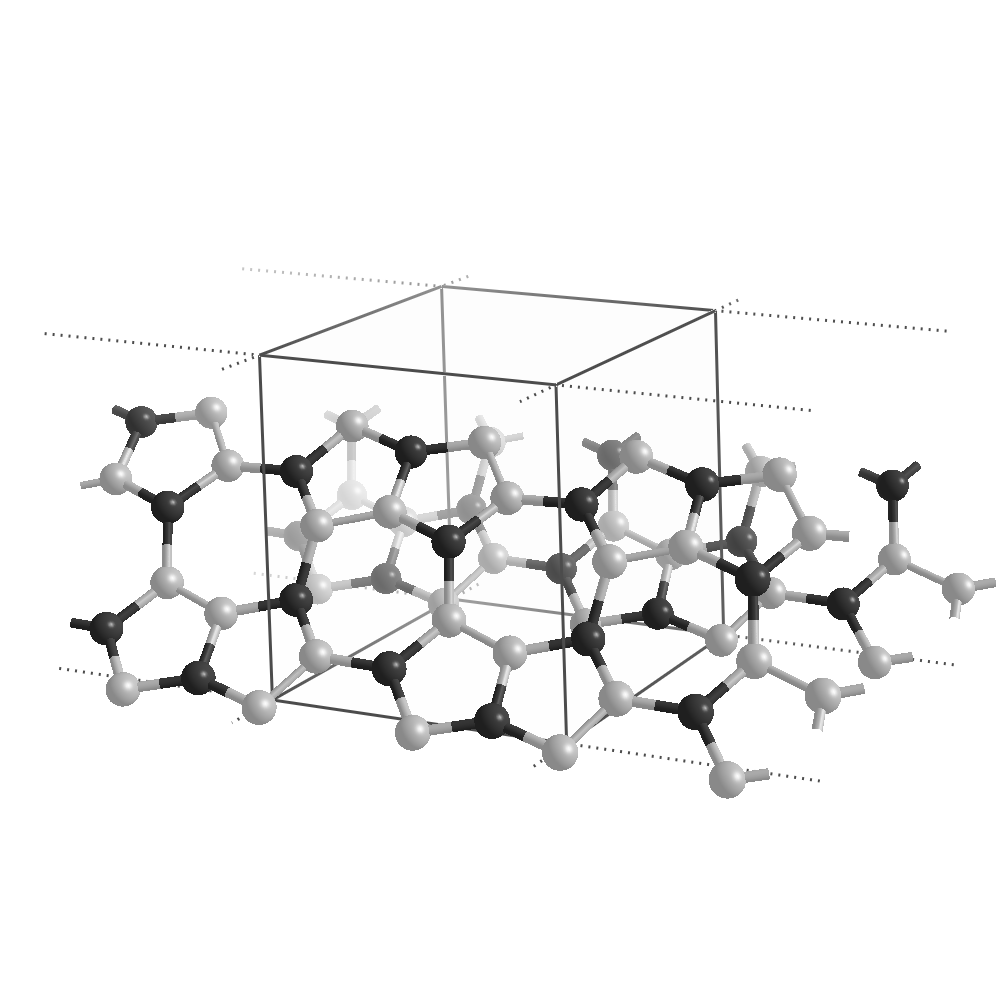
\includegraphics[clip,scale=0.3]{Figures/16structure.png}%
}

\caption{Example of the crystal structures used. C atoms are in black and N atoms in white. (A): Crystal sctructure with 8 atoms per cell. (B): Crystal structure with 16 atoms per cell.}

\end{figure}
\newpage
\subsection{Orbital Energies}
For calculating the overlap matrix (eq. \ref{ovrlap} ff.) the gaussian width $\alpha_i$ was originaly only dependent on the covalent radius of the respective atom type. This was further modified to respect the orbital eigenenergy of the respective orbital (eq. \ref{eq:const}). The values used were gathered from the NIST Atomic Reference Data for Electronic Stucture Calculations.

\begin{table}[h!]
\center
\label{table:energies}
\begin{tabular}{c|c|c}
            & \textbf{C} & \textbf{N} \\ \hline
2s {[}eV{]} & -0.500866  & -0.676151  \\ \hline
2p {[}eV{]} & -0.199186  & -0.266297 
\end{tabular}
\caption{2s and 2p orbital eigenenergies of N and C.}
\end{table}

The constant $C$ in (eq. \ref{eq:const}) was experimentally determined. To obtain a good resolution in comparing the fingerprints, the entries of the fingerprints should be reasonably large, but not to close to each other. One can see the effect of the constant $C$ out of (eq. \ref{eq:const}) by plotting the constant vs. the entries of the fingerprint.
With plots as seen in Figure \ref{fig:const} one can determine approximate boundaries for the constant. The entries should be reasonably distinct but still large enough to get a good resolution. The fine tuning was then done via maximizing the prediction accuracy. The final value used for all calculation was then $C=0.19$.


\begin{figure}[h]

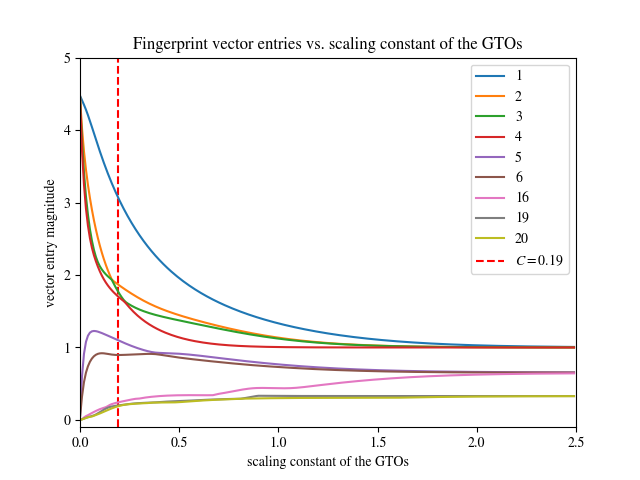
\includegraphics[width=\linewidth]{Figures/fpentry.png}
\caption{Plot of the fingerprint vector entries enumerated vs. the scaling constant of the GTO width.}
\label{fig:const} 
\end{figure}

\newpage
\section{Results}
\subsection{Landmark structures}

To calculate the landmark structures out of the fingerprints, we used a direct implementation of the maximum volume simplex method \cite{Behnam2020}. The task of this method should be to evaluate all atomar fingerprints given to it, and return the most distinct environments. These most distinct environments should furthermore each describe a different case of possible atomic environment regarding number of nearest neighbours (ligancy or coordination number) and type of nearest neighbours and their permutations. The method was evaluated on the set of 99 crystals with 8 atoms per crystal. Out of these 792 possible environments, the algorithm constructed a maximum volume simplex with 101 corners. A few of these landmark environments can be seen in Figure \ref{fig:landmarks1}, Figure \ref{fig:landmarks2}, Figure \ref{fig:landmarks3} and Figure \ref{fig:landmarks4}. The center atom is always either colored red for carbon and yellow for nitrogen in these depictions. Some of the atomic bonds were omited selectivly for visual clarity.


\begin{figure}[h!]

\center
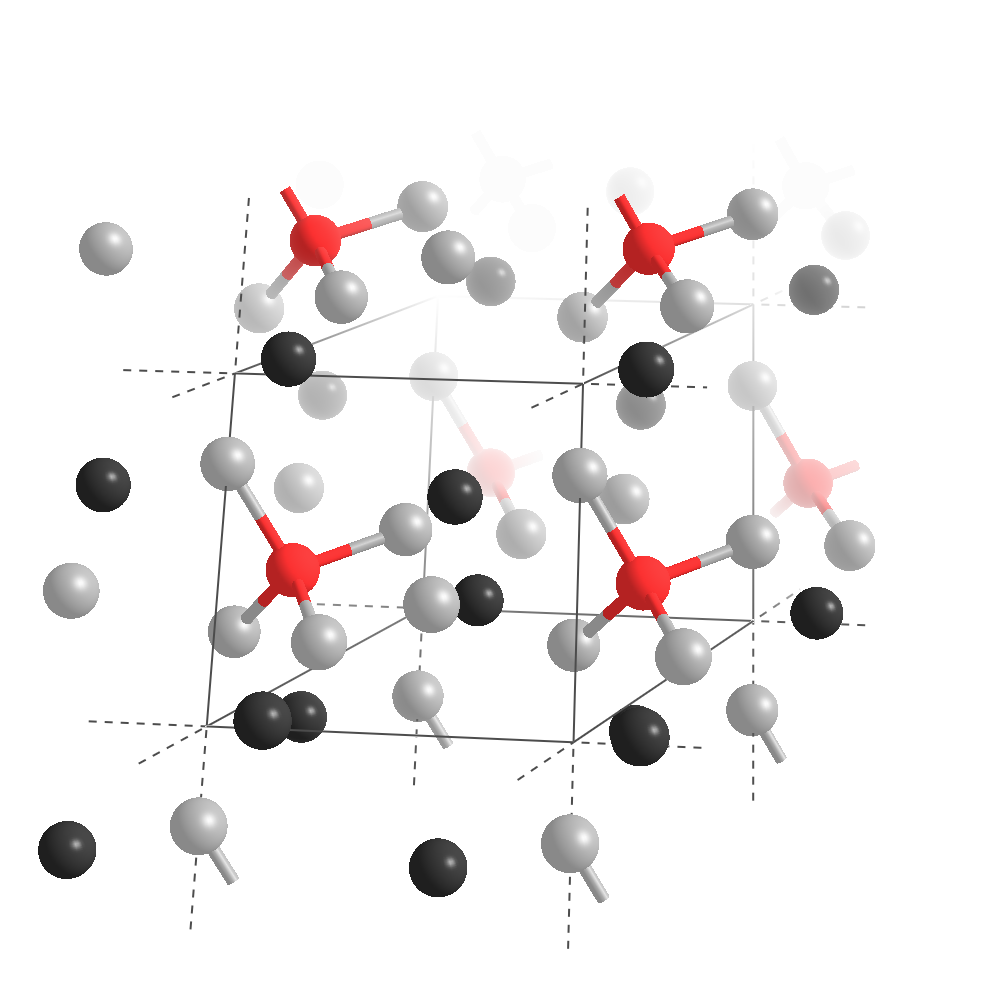
\includegraphics[width=\linewidth]{Figures/landmark1.png}
\caption{Landmark structure: Four times coordinated carbon with 4 nitrogen neighbours; black: carbon; white: nitrogen; red: carbon center atom. }
\label{fig:landmarks1}
\end{figure}

\begin{figure}[p]
\center
\subfloat[Once cooredinated nitrogen]{%
  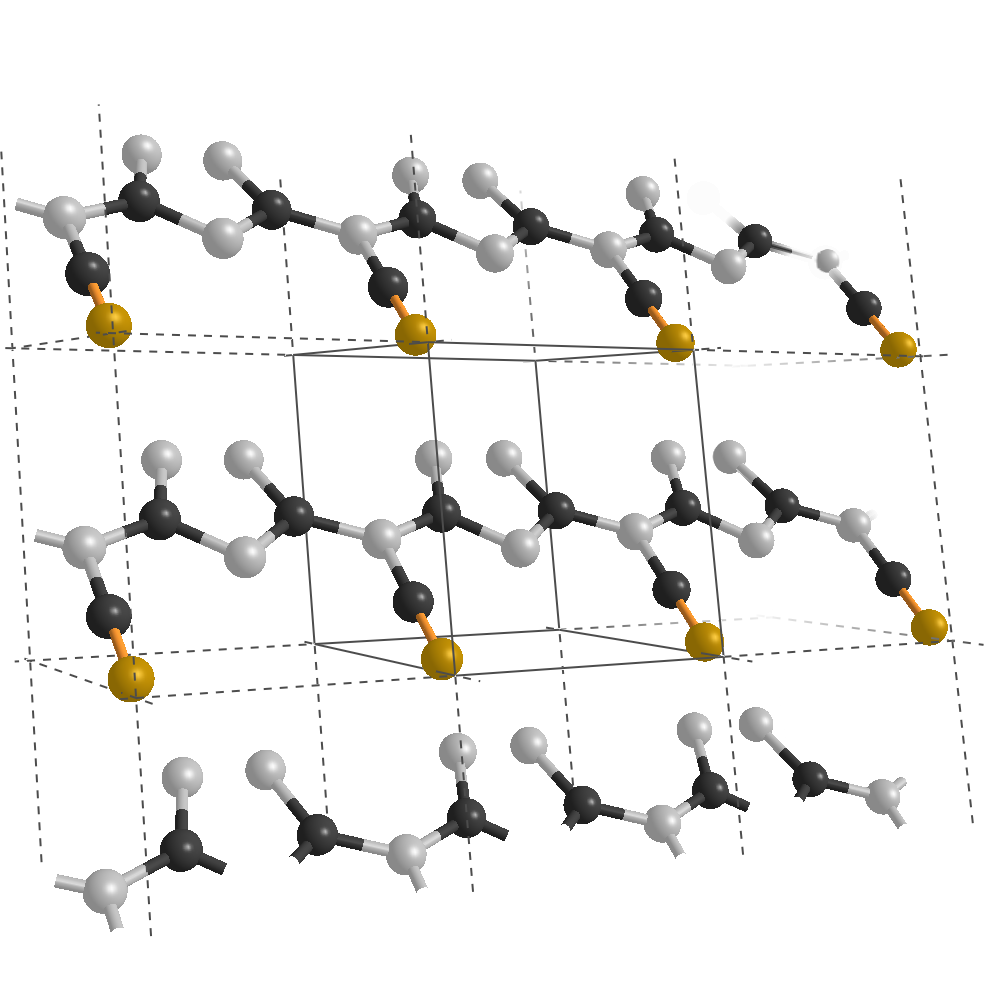
\includegraphics[clip,scale=0.3]{Figures/landmark2.png}%
}

\subfloat[Twice coordinated carbon]{%
  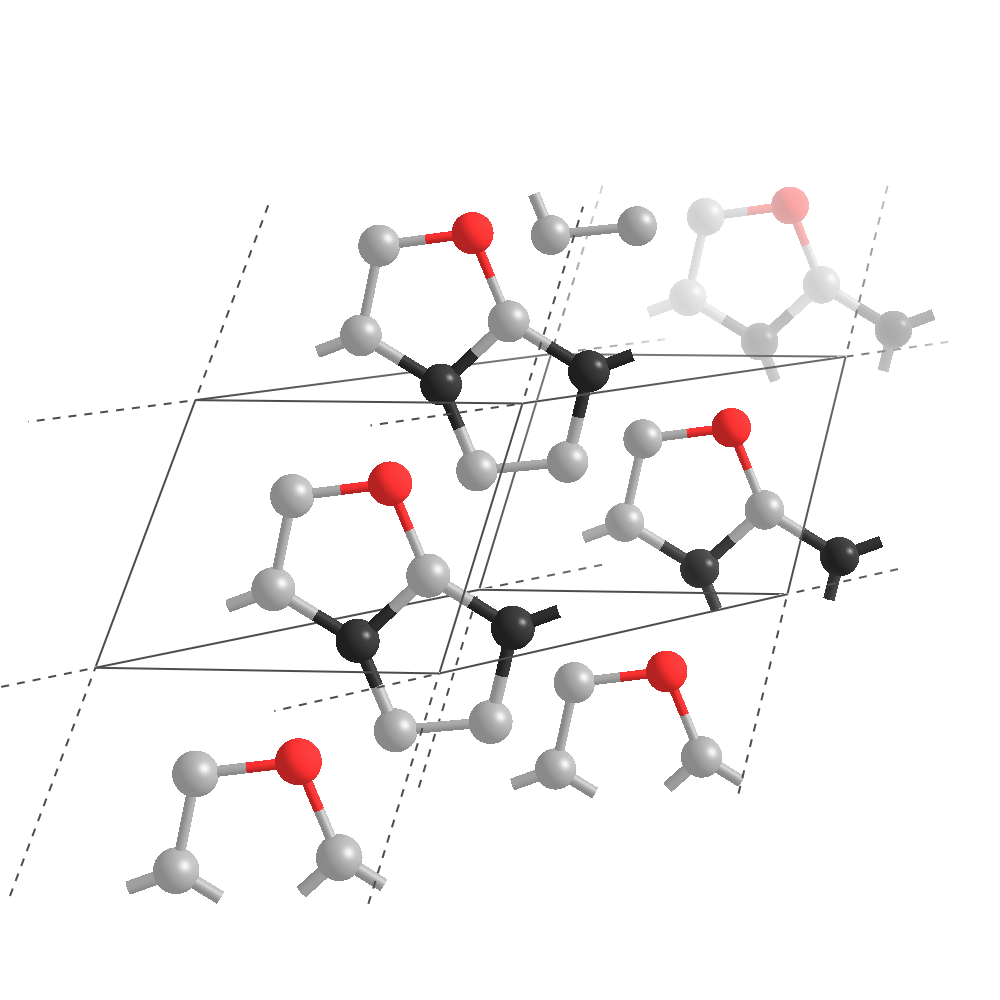
\includegraphics[clip,scale=0.3]{Figures/landmark3.png}%
}

\caption{Landmark structures: black: carbon; white: nitrogen; red: carbon center atom, yellow: nitrogen center atom}
\label{fig:landmarks2}

\end{figure}

\begin{figure}[p]
\center
\subfloat[three times cooredinated nitrogen with 3 carbon and 1 nitrogen neighbour]{%
  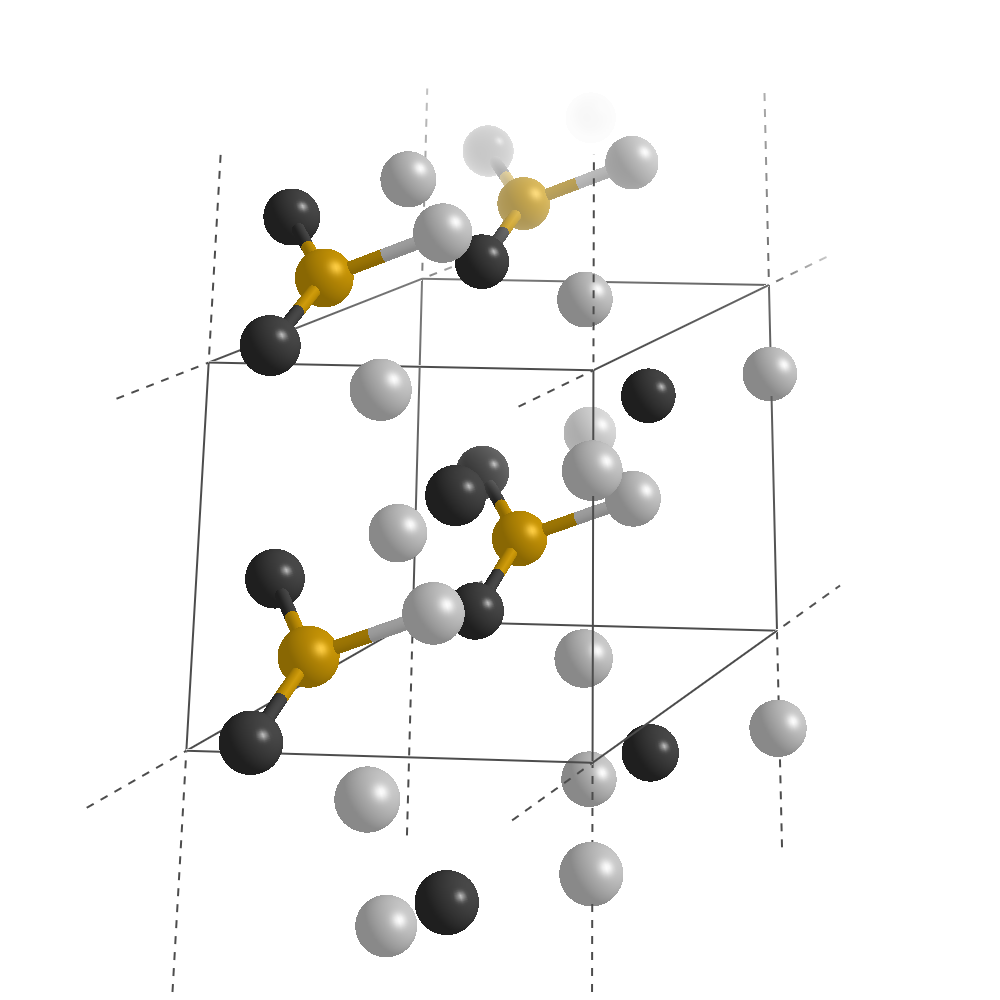
\includegraphics[clip,scale=0.3]{Figures/landmark4.png}%
}

\subfloat[three times cooredinated nitrogen with 3 carbon neighbours]{%
  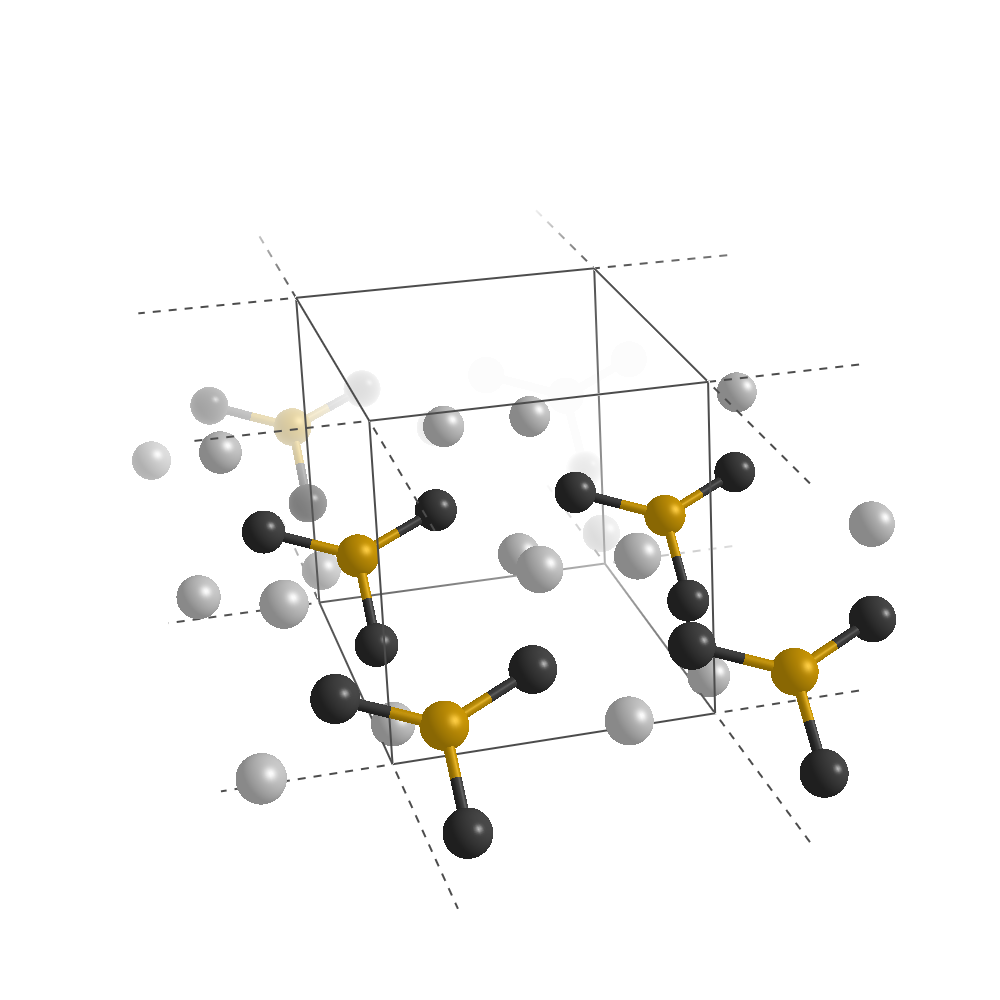
\includegraphics[clip,scale=0.3]{Figures/landmark5.png}%
}

\caption{Landmark structures: black: carbon; white: nitrogen; red: carbon center atom, yellow: nitrogen center atom}
\label{fig:landmarks3}

\end{figure}

\begin{figure}[p]
\center
\subfloat[twice coordinated carbon with 2 nitrogen neighbours]{%
  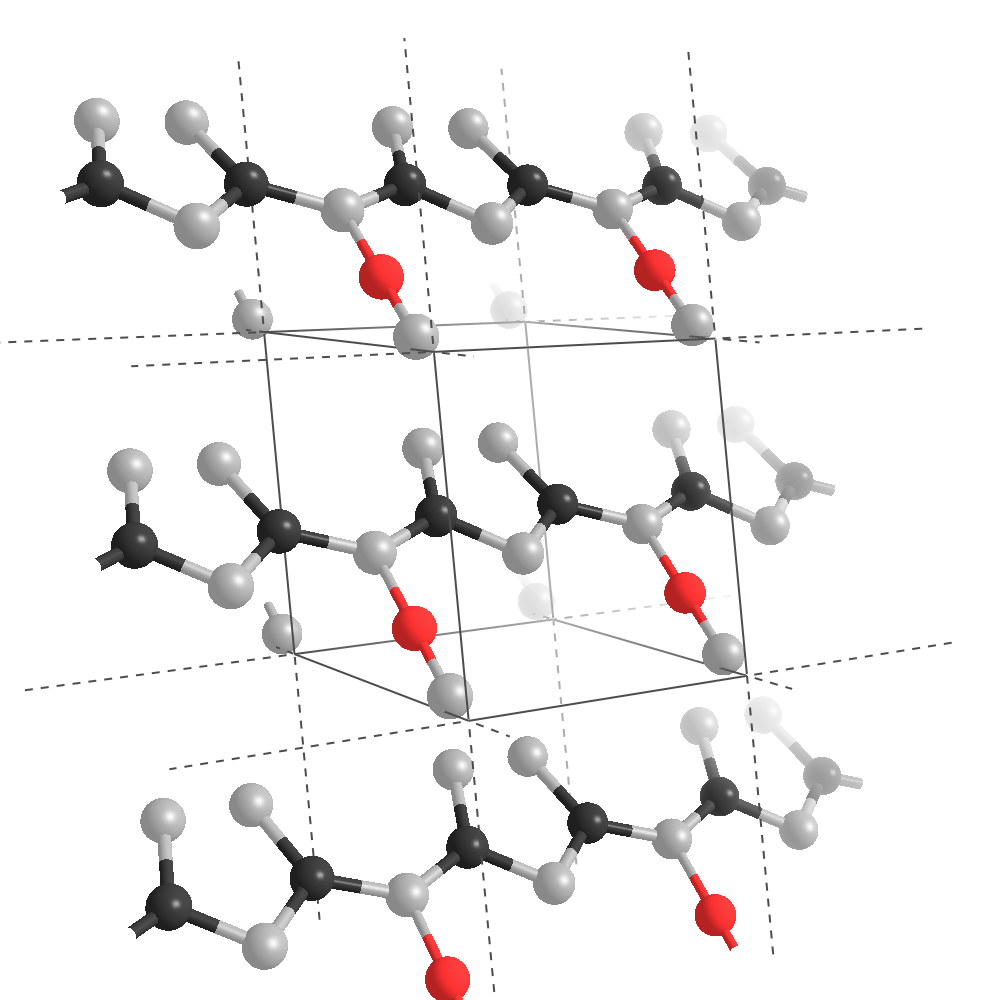
\includegraphics[clip,scale=0.3]{Figures/landmark6.png}%
}

\subfloat[three times cooredinated carbon with 3 nitrogen neighbours]{%
  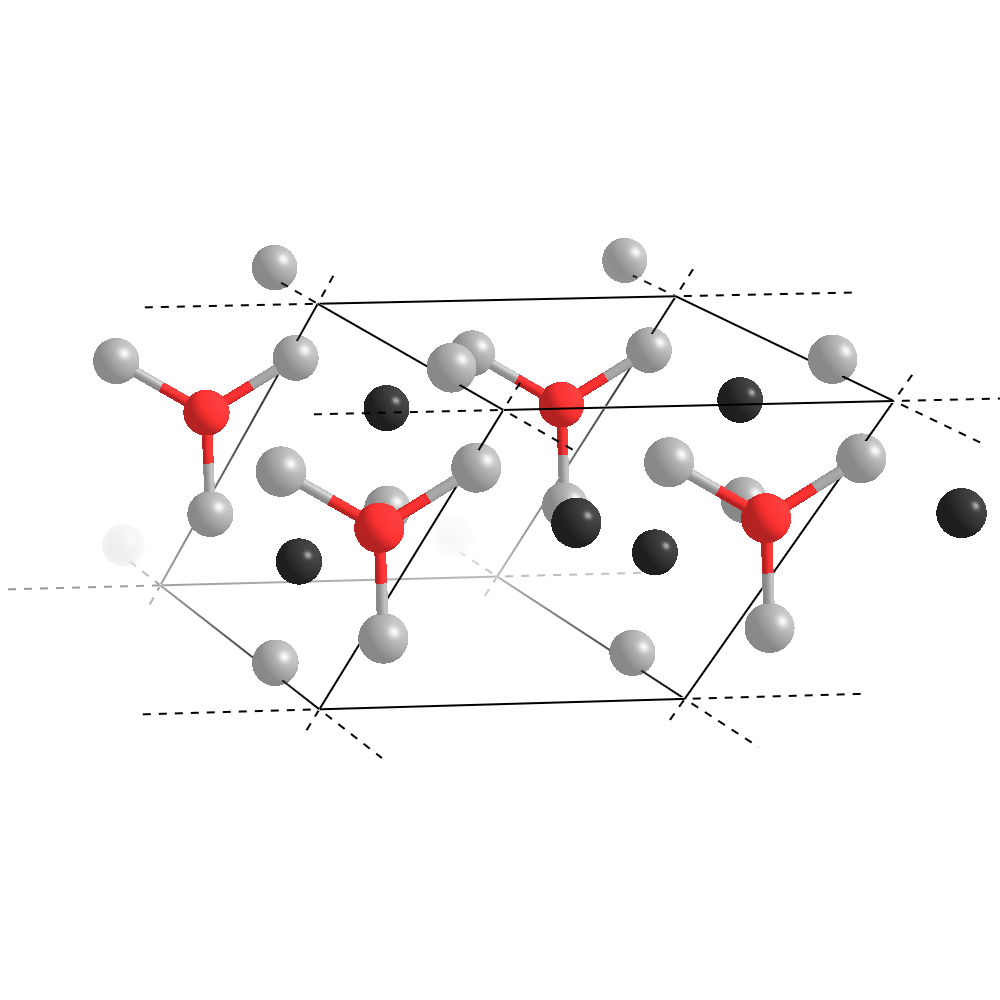
\includegraphics[clip,scale=0.3]{Figures/landmark7.png}%
}

\caption{Landmark structures: black: carbon; white: nitrogen; red: carbon center atom, yellow: nitrogen center atom}
\label{fig:landmarks4}

\end{figure}


\newpage
\subsection{Classification}
The classification was done in a relativly simple way. First, the \emph{trainings fingerprints} are calculated with the procedures mentioned earlier in this text. Then, the maximum simplex method is used to identify 101 landmark fingerprints. Of these landmark fingerprints, the type of center atom is stored aswell. Now, any atomar fingerprint can be compared to the landmark fingerprint via the euclidian distance. If the closest corner to our atom is a carbon, it predicts carbon. If the closest corner is a nitrogen, it predicts nitrogen.\\
\subsubsection{Training on eight atom crystals}
We trained our model first on a set of 99 configurations with 8 atoms per cell (3 Carbon and 5 Nitrogen). This was then validated on a set of 4949 crystals with 16 atoms per cell (6 carbon and 10 nitrogen) which gives us about 79'000 different environments to classify. The results of this procedure can be seen in Table \ref{table:res1}. 

\begin{table}[h!]
\center
\begin{tabular}{c|c|c|c}
classification & correct & false & correct (relative) \\ \hline
C              & 26497   & 4064  & 0.867              \\ \hline
N              & 45426   & 3197  & 0.934              \\ \hline
Total          & 71923   & 7261  & 0.908             
\end{tabular}
\caption{Classification results for the 4949 carbon nitrate crystals with 16 atoms per cell (79184 atoms in total) trained on 99 crystals with 8 atoms per cell.}
\label{table:res1}
\end{table}

One can see in Table \ref{table:res1} that the classification accuracy for carbon is considerably lower than that for nitrogen. The reason for this effect lies probably within the fact, that our trainings data contains about 1.6 times more nitrogen samples than carbon samples. So our model "knows" the nitrogen case better.

\subsubsection{Training on 16 atom crystals}
Next, we trained our model on a random selction of 63 16 atom crystals out of the 4949 crystals at our disposal. Then we classified the whole set of 16 atom crystals. The results can be seen in Table \ref{table:res2}.

\begin{table}[h!]
\center
\begin{tabular}{c|c|c|c}
classification & correct & false & correct (relative) \\ \hline
C              & 21151   & 3917  & 0.844              \\ \hline
N              & 45573   & 8543  & 0.842              \\ \hline
Total          & 66724   & 12460  & 0.843             
\end{tabular}
\caption{Classification results for the 4949 carbon nitrate crystals with 16 atoms per cell (79184 atoms in total) trained on 63 crystals with 16 atoms per cell.}
\label{table:res2}
\end{table}

Surprisingly, the accuracy is worse than before. Apparently training on a different (smaller) number of atoms per cell yielded better results than on training on the same. This of course can't be taken at face value since evaluating and comparing performance of machine learning methods is a very involved process which we will not get into in this report.



\subsection{Comparing to Supervised Learning with Random Forests}
Random Forests are intresting models for classification, since they require little configuration for reasonable predictions. The algorithm was first proposed by \citeauthor{Ho1995} \cite{Ho1995} and then extenden by \citeauthor{Breiman2001} \cite{Breiman2001}. It is a typical example of supervised learning, mapping input to output based on example input-ouput pairs. In our case, the example pairs are the either carbon or nitrogen labeled fingerprints in the trainings set.
The alrogrithm is very fast to train and very fast to validate. Training on a set of 52000 vectors willth 500 estimators on a consumer computer takes about 2 minutes. Once trained, the method can classify the 25000 fingerprints in a matter of seconds. We used the implementation of the Random Forest Classifier implemented for Python in scikit-learn by \citeauthor{scikit} \cite{scikit}. 

\begin{table}[h!]
\center
\begin{tabular}{c|c|c|c}
classification & correct & false & correct (relative) \\ \hline
C              & 8383   & 1475  & 0.850              \\ \hline
N              & 16128   & 407  & 0.975              \\ \hline
Total          & 24511   & 1881  & 0.929             
\end{tabular}
\caption{Classification results for the 26395 environments of the 16 atom structures averaged over 10 tries.}
\label{table:res3}
\end{table}

The results in Table \ref{table:res3} show an even greater divide between nitrogen and carbon which is again not surprising due to the imbalance of carbon to nitrogen in the training data. The Random Forest classifies the fingerprint vectors very well with an accuracy of about 93\% out of the box. This shows that the information we are looking for is clearly available in the fingerprint vector. The problem of Random Forests and supervised learning in general for our purposes is that it acts more or less as a black box. We can not deduce or induce physical meaning into or out of the work done by the Random Forest easily. It is however a powerful tool to see if the data contains the information we are looking for.

\section{Conclusion}
Being able to deduct the type of elements present in crystals just by looking at the atomic positions is something very useful in solid state physics. We demonstrated that the fingerprinting method and the maximum simplex method can be used to determine such quantities. The limitations with this method so far are that we are only looking at two different species of atoms and are therefore quite limited in what we can do. This could naturaly be extended to more atomic species, since the only parameters used were physical constants like the orbital eigenenergies and the covalent radii which are quantities very well known for most of the periodic table. There is also already a huge amount of data available to test and improve the method to suit tasks like classifying structures with more than two different kinds of atoms. Integrating both analytical methods such as the maximum simplex method and stochastic methods such as random forests and supervised learning in general shows huge potential in solid state physics.

% Training set size: 52789
% Validation set size: 26395
% (79184,)
% (79184, 400)
% [Parallel(n_jobs=1)]: Using backend SequentialBackend with 1 concurrent workers.
% [Parallel(n_jobs=1)]: Done 500 out of 500 | elapsed:  3.1min finished
% [Parallel(n_jobs=1)]: Using backend SequentialBackend with 1 concurrent workers.
% [Parallel(n_jobs=1)]: Done 500 out of 500 | elapsed:    3.2s finished
% The ratio of correct guesses is: 0.9227475941501857
% [[ 8316  1610]
%  [  429 16039]]
%% Chapter Template

\chapter{Implementation and Results} % Main chapter title

\label{Chapter2} % Change X to a consecutive number; for referencing this chapter elsewhere, use \ref{ChapterX}

%----------------------------------------------------------------------------------------
%	SECTION 1
%----------------------------------------------------------------------------------------

\section{Implementation}
The code base worked with, was a direct Fortran90 implementation of the fingerprint algorithm proposed by \cite{Zhu2016}. The compiler used for all computation was the GNU Fortran compiler \cite{gnufortran}.

\subsection{Data}
The structures used for evaluating our methods were carbon-nitrate crystals. The data contained the positions of the atoms in cartesian coordinates and the lattice vectors of the unit cell. We thank Prof. Alireza Ghasemi for providing us with the data base of carbon-nitate structures that we have analysed.


\begin{figure}[p]
\center
\label{fig:structures}
\subfloat[8 atom unit cell]{%
  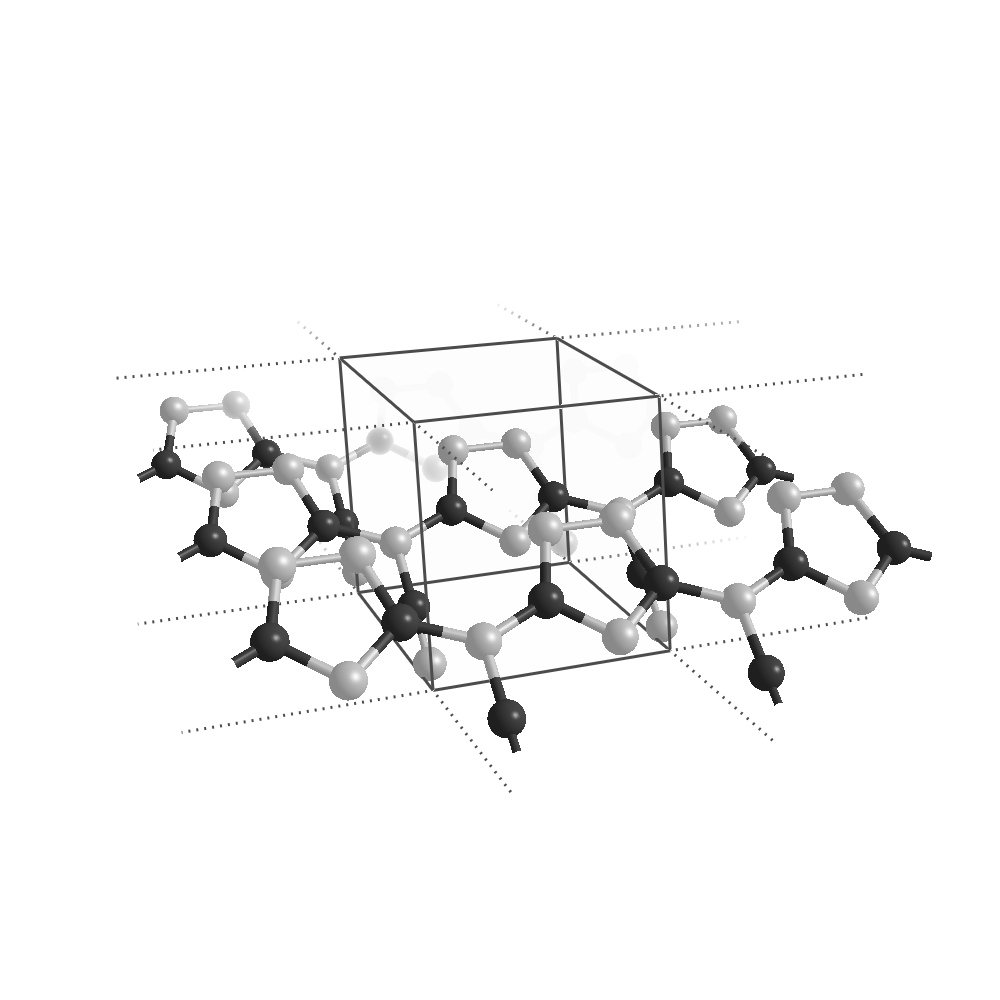
\includegraphics[clip,scale=0.3]{Figures/8structure.png}%
}

\subfloat[16 atom unit cell]{%
  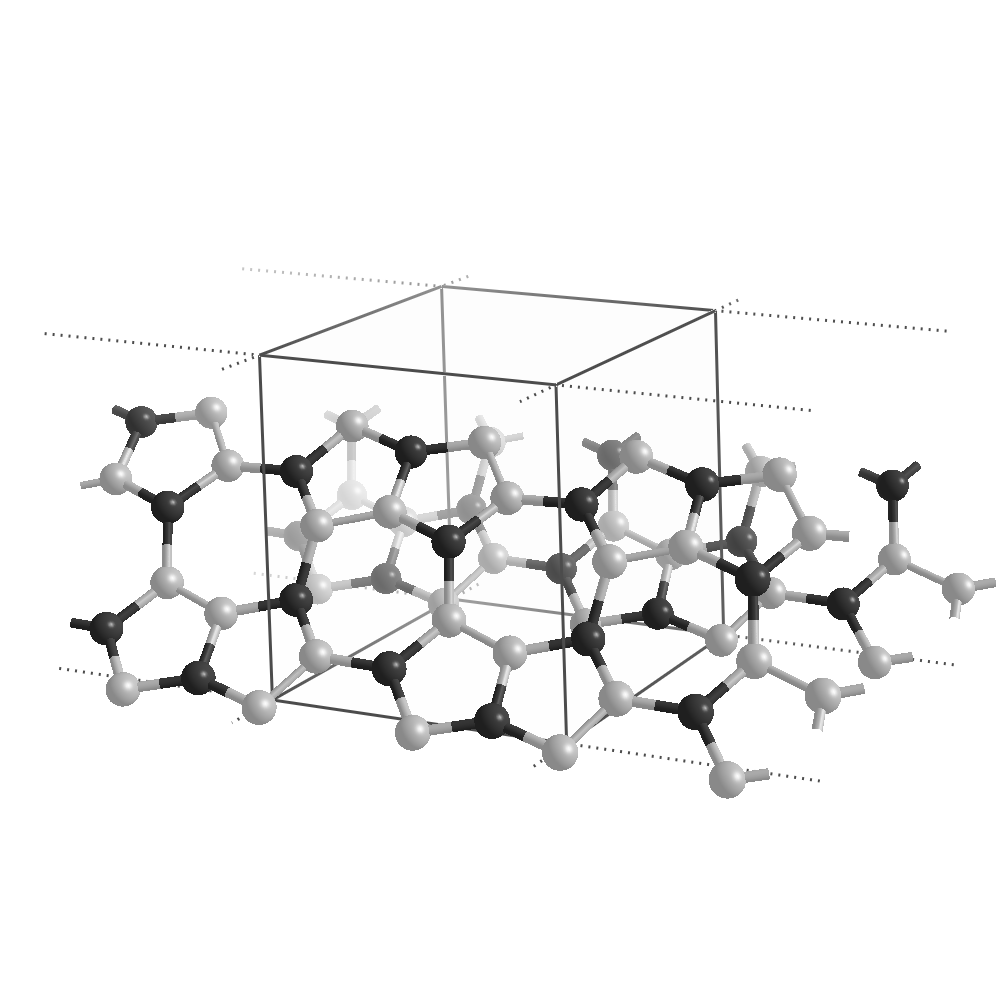
\includegraphics[clip,scale=0.3]{Figures/16structure.png}%
}

\caption{Example of the crystal structures used. C atoms are in black and N atoms in white. (A): Crystal sctructure with 8 atoms per cell. (B): Crystal structure with 16 atoms per cell.}

\end{figure}
\newpage
\subsection{Orbital Energies}
For calculating the overlap matrix (eq. \ref{ovrlap} ff.) the gaussian width $\alpha_i$ was originaly only dependent on the covalent radius of the respective atom type. This was further modified to respect the orbital eigenenergy of the respective orbital (eq. \ref{eq:const}). The values used were gathered from the NIST Atomic Reference Data for Electronic Stucture Calculations.

\begin{table}[h!]
\center
\label{table:energies}
\begin{tabular}{c|c|c}
            & \textbf{C} & \textbf{N} \\ \hline
2s {[}eV{]} & -0.500866  & -0.676151  \\ \hline
2p {[}eV{]} & -0.199186  & -0.266297 
\end{tabular}
\caption{2s and 2p orbital eigenenergies of N and C.}
\end{table}

The constant $C$ in (eq. \ref{eq:const}) was experimentally determined. To obtain a good resolution in comparing the fingerprints, the entries of the fingerprints should be reasonably large, but not to close to each other. One can see the effect of the constant $C$ out of (eq. \ref{eq:const}) by plotting the constant vs. the entries of the fingerprint.
With plots as seen in Figure \ref{fig:const} one can determine approximate boundaries for the constant. The entries should be reasonably distinct but still large enough to get a good resolution. The fine tuning was then done via maximizing the prediction accuracy. The final value used for all calculation was then $C=0.19$.


\begin{figure}[h]

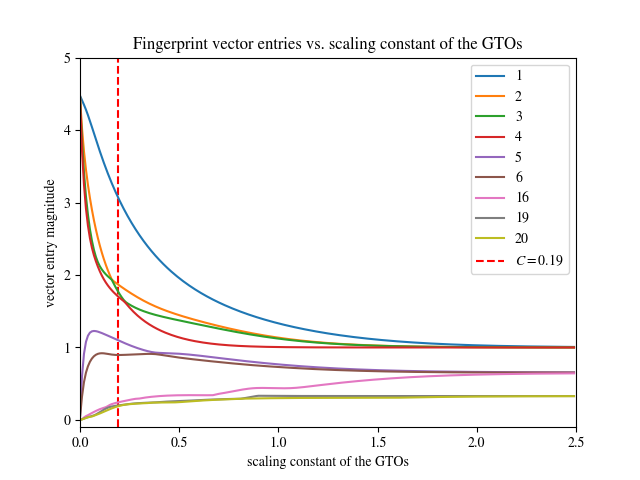
\includegraphics[width=\linewidth]{Figures/fpentry.png}
\caption{Plot of the fingerprint vector entries enumerated vs. the scaling constant of the GTO width.}
\label{fig:const} 
\end{figure}

\newpage
\section{Results}
\subsection{Landmark structures}

To calculate the landmark structures out of the fingerprints, we used a direct implementation of the maximum volume simplex method \cite{Behnam2020}. The task of this method should be to evaluate all atomar fingerprints given to it, and return the most distinct environments. These most distinct environments should furthermore each describe a different case of possible atomic environment regarding number of nearest neighbours (ligancy or coordination number) and type of nearest neighbours and their permutations. The method was evaluated on the set of 99 crystals with 8 atoms per crystal. Out of these 792 possible environments, the algorithm constructed a maximum volume simplex with 101 corners. A few of these landmark environments can be seen in Figure \ref{fig:landmarks1}, Figure \ref{fig:landmarks2}, Figure \ref{fig:landmarks3} and Figure \ref{fig:landmarks4}. The center atom is always either colored red for carbon and yellow for nitrogen in these depictions. Some of the atomic bonds were omited selectivly for visual clarity.


\begin{figure}[h!]

\center
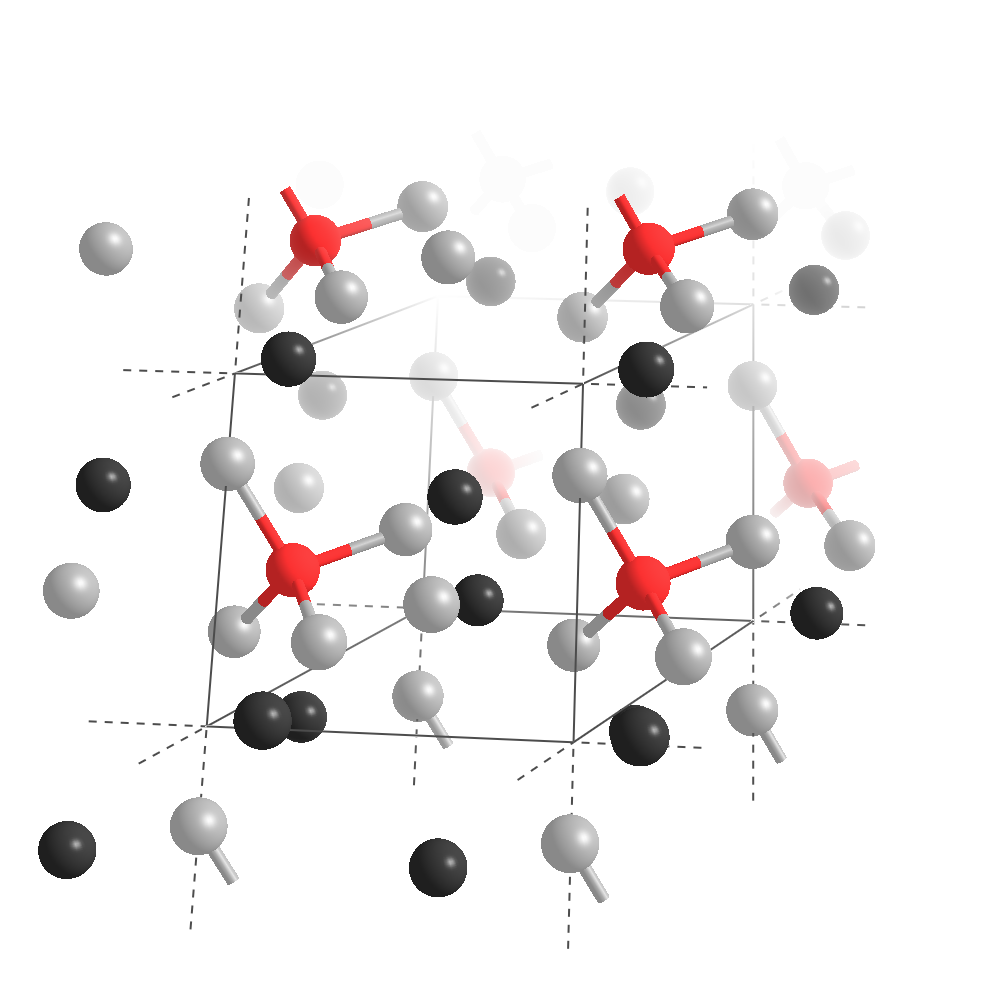
\includegraphics[width=\linewidth]{Figures/landmark1.png}
\caption{Landmark structure: Four times coordinated carbon with 4 nitrogen neighbours; black: carbon; white: nitrogen; red: carbon center atom. }
\label{fig:landmarks1}
\end{figure}

\begin{figure}[p]
\center
\subfloat[Once cooredinated nitrogen]{%
  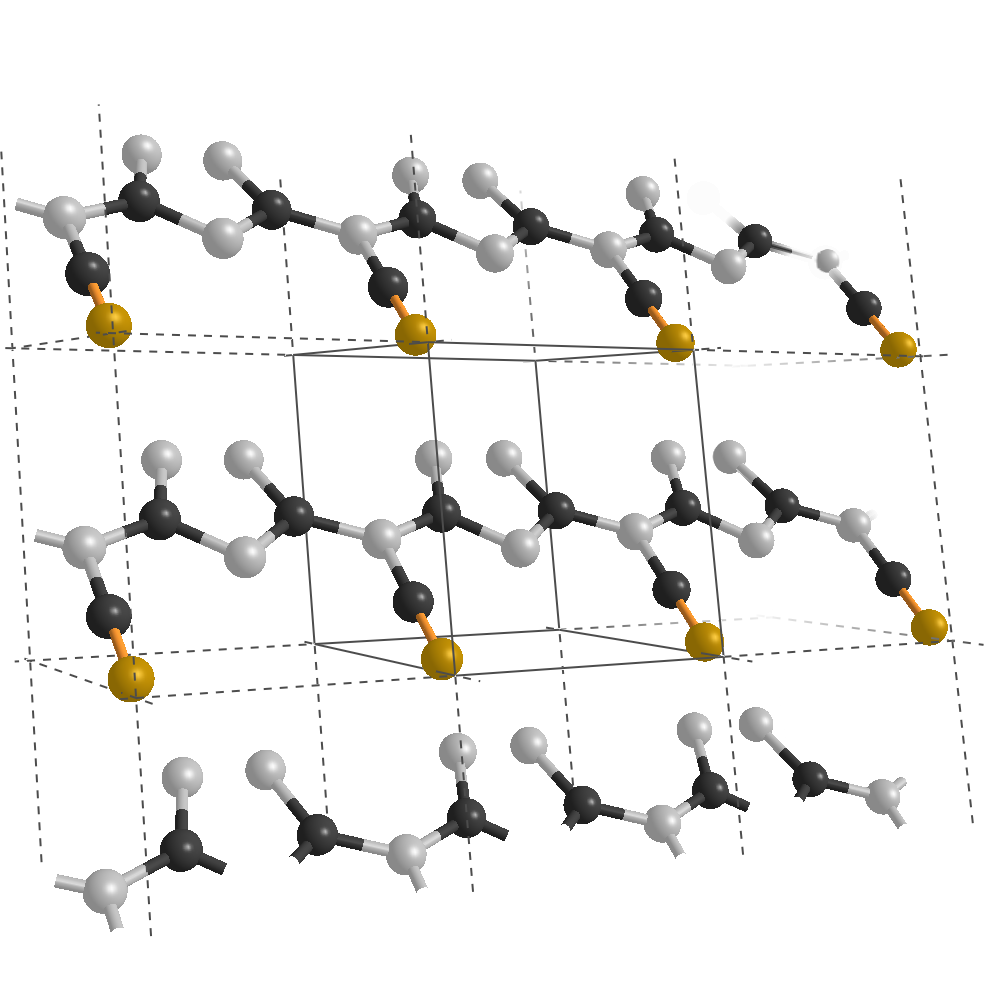
\includegraphics[clip,scale=0.3]{Figures/landmark2.png}%
}

\subfloat[Twice coordinated carbon]{%
  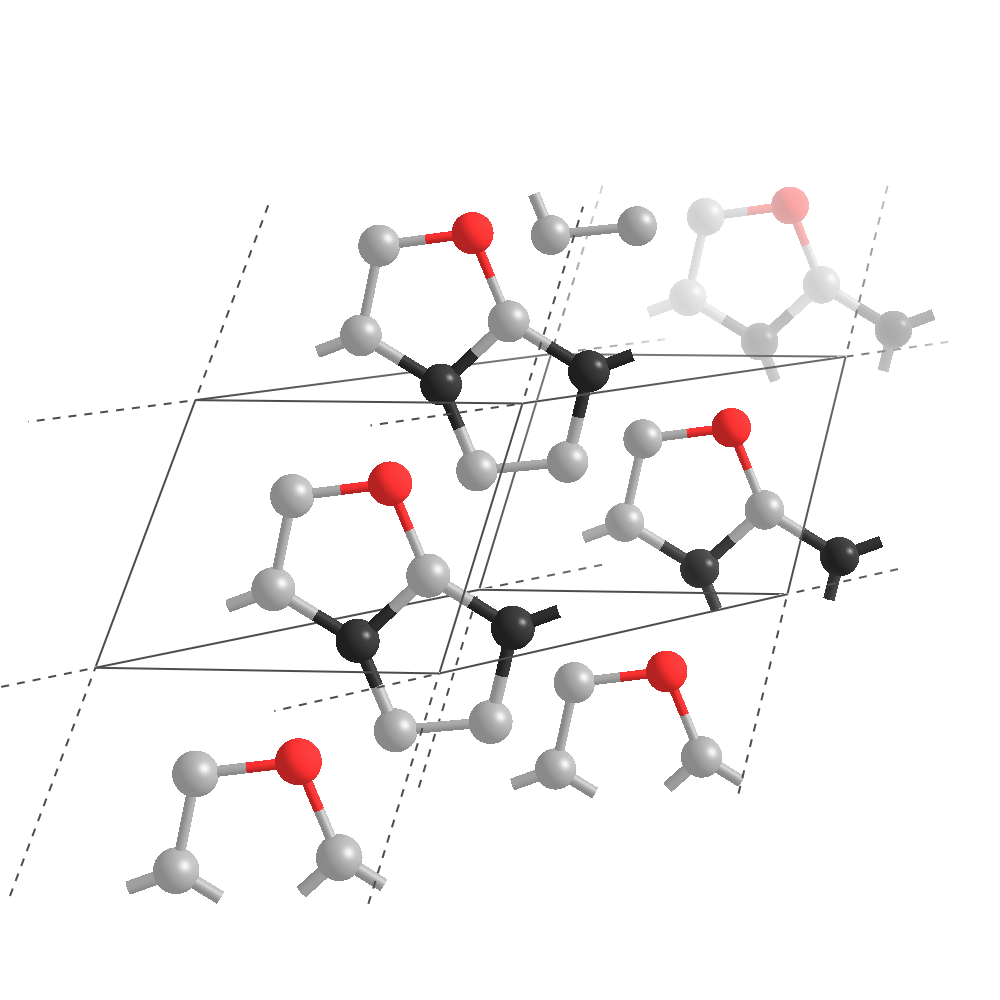
\includegraphics[clip,scale=0.3]{Figures/landmark3.png}%
}

\caption{Landmark structures: black: carbon; white: nitrogen; red: carbon center atom, yellow: nitrogen center atom}
\label{fig:landmarks2}

\end{figure}

\begin{figure}[p]
\center
\subfloat[three times cooredinated nitrogen with 3 carbon and 1 nitrogen neighbour]{%
  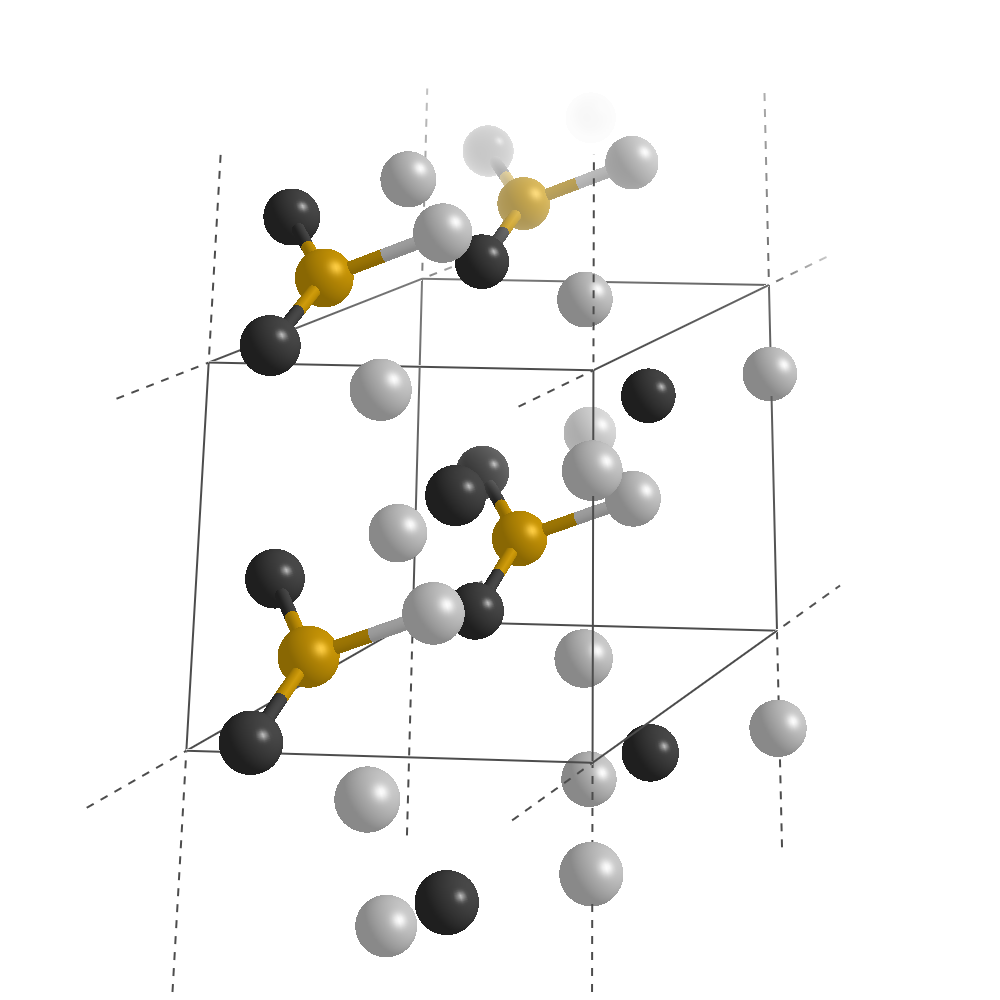
\includegraphics[clip,scale=0.3]{Figures/landmark4.png}%
}

\subfloat[three times cooredinated nitrogen with 3 carbon neighbours]{%
  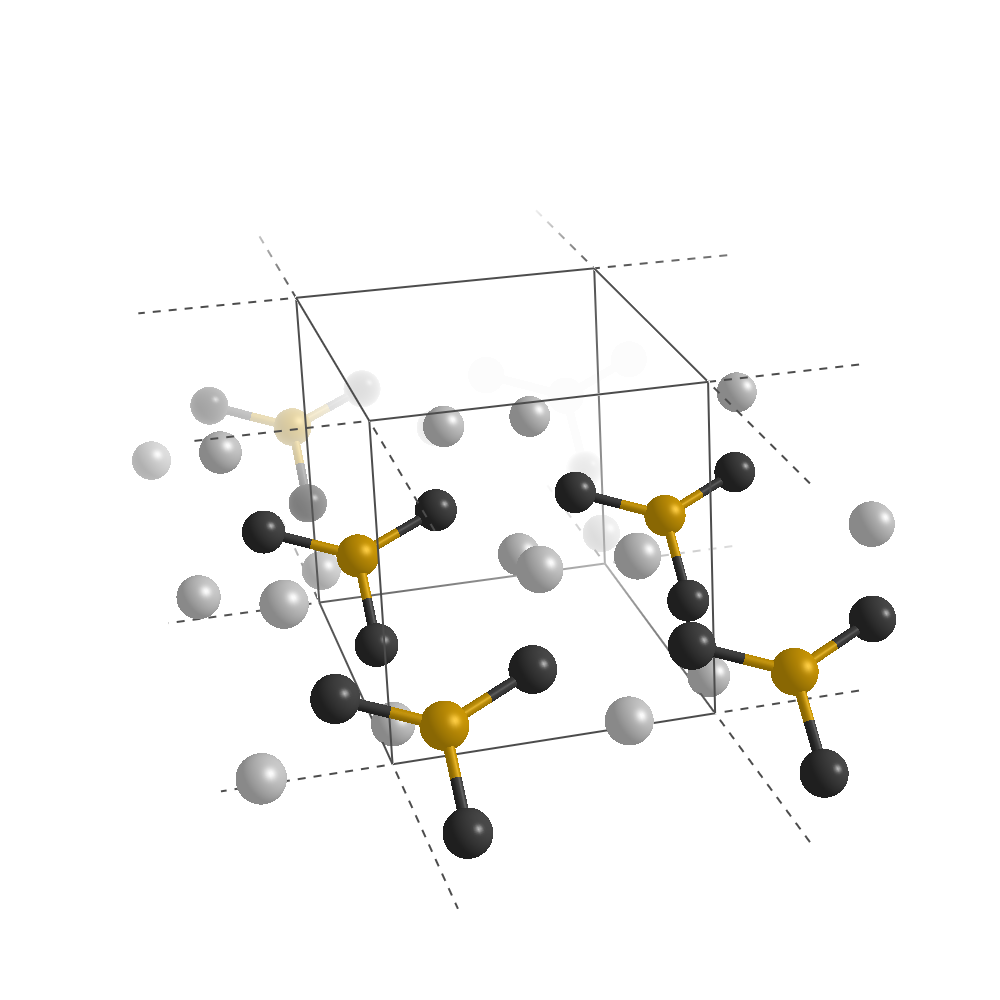
\includegraphics[clip,scale=0.3]{Figures/landmark5.png}%
}

\caption{Landmark structures: black: carbon; white: nitrogen; red: carbon center atom, yellow: nitrogen center atom}
\label{fig:landmarks3}

\end{figure}

\begin{figure}[p]
\center
\subfloat[twice coordinated carbon with 2 nitrogen neighbours]{%
  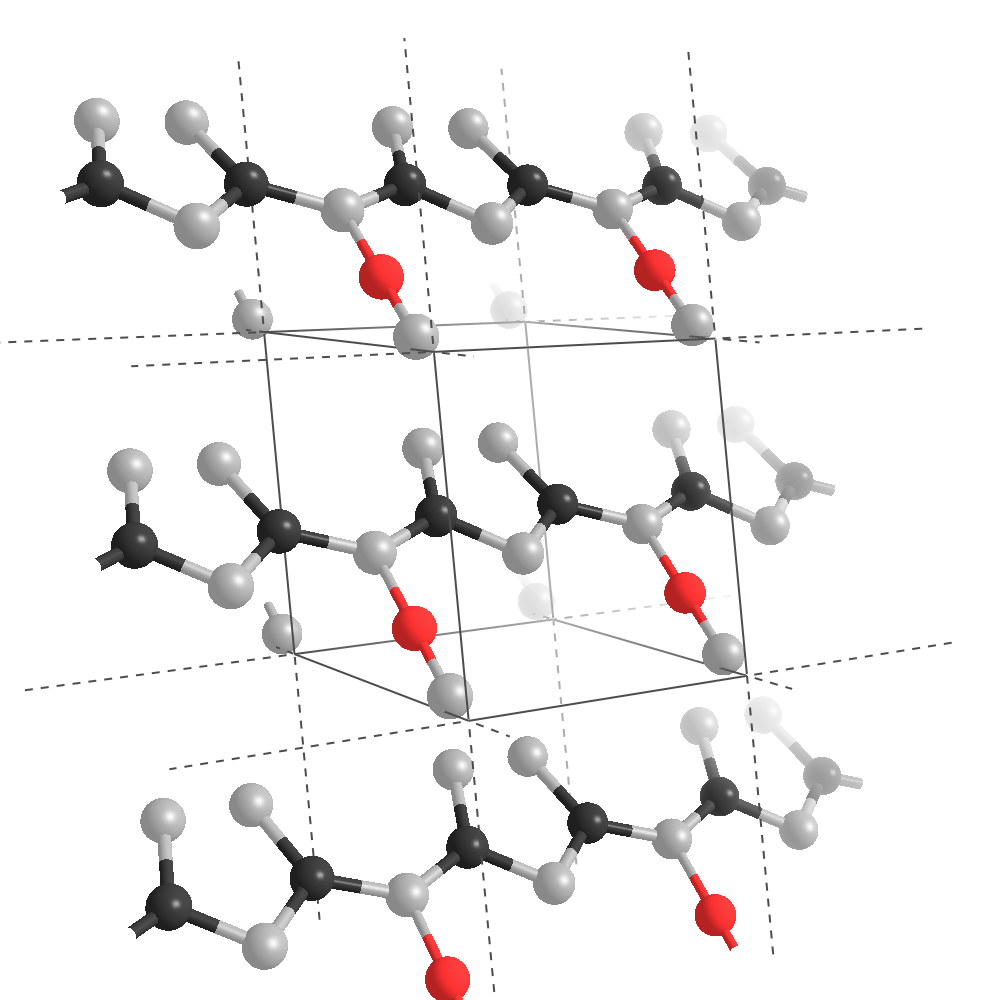
\includegraphics[clip,scale=0.3]{Figures/landmark6.png}%
}

\subfloat[three times cooredinated carbon with 3 nitrogen neighbours]{%
  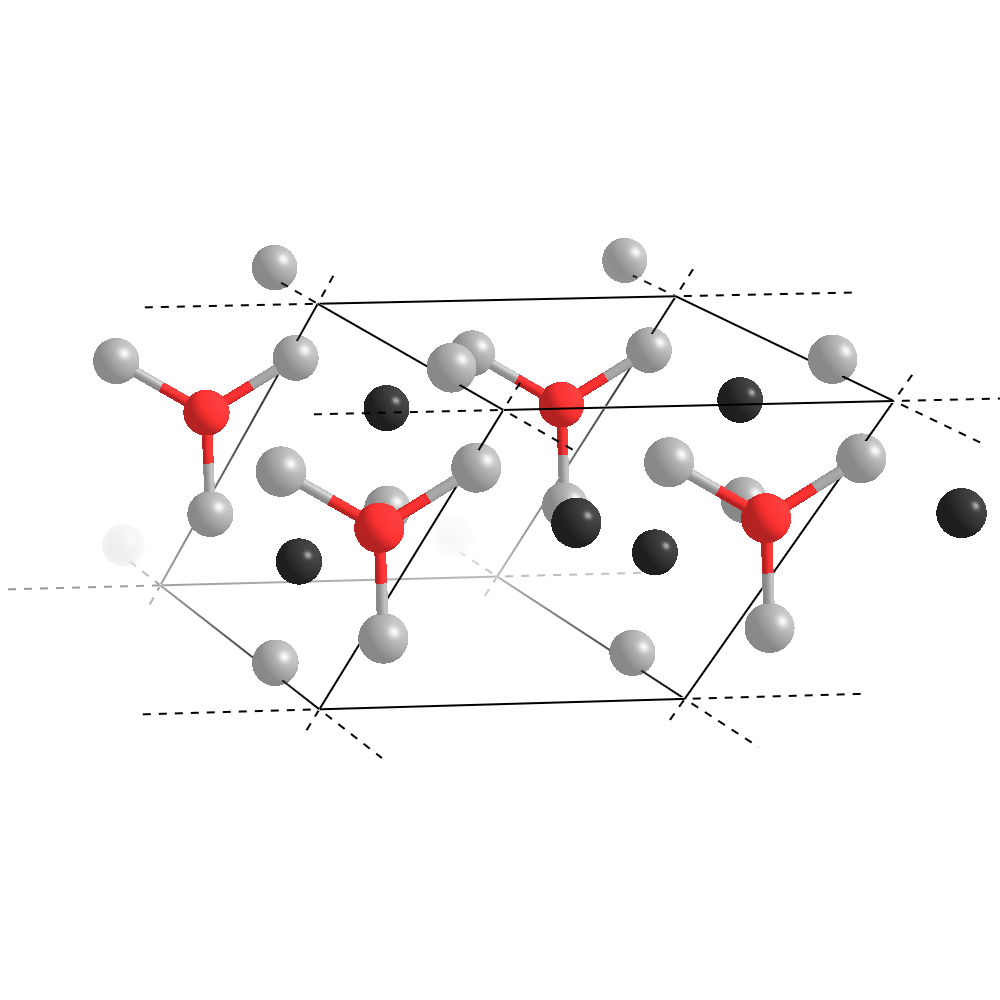
\includegraphics[clip,scale=0.3]{Figures/landmark7.png}%
}

\caption{Landmark structures: black: carbon; white: nitrogen; red: carbon center atom, yellow: nitrogen center atom}
\label{fig:landmarks4}

\end{figure}


\newpage
\subsection{Classification}
The classification was done in a relativly simple way. First, the \emph{trainings fingerprints} are calculated with the procedures mentioned earlier in this text. Then, the maximum simplex method is used to identify 101 landmark fingerprints. Of these landmark fingerprints, the type of center atom is stored aswell. Now, any atomar fingerprint can be compared to the landmark fingerprint via the euclidian distance. If the closest corner to our atom is a carbon, it predicts carbon. If the closest corner is a nitrogen, it predicts nitrogen.\\
\subsubsection{Training on eight atom crystals}
We trained our model first on a set of 99 configurations with 8 atoms per cell (3 Carbon and 5 Nitrogen). This was then validated on a set of 4949 crystals with 16 atoms per cell (6 carbon and 10 nitrogen) which gives us about 79'000 different environments to classify. The results of this procedure can be seen in Table \ref{table:res1}. 

\begin{table}[h!]
\center
\begin{tabular}{c|c|c|c}
classification & correct & false & correct (relative) \\ \hline
C              & 26497   & 4064  & 0.867              \\ \hline
N              & 45426   & 3197  & 0.934              \\ \hline
Total          & 71923   & 7261  & 0.908             
\end{tabular}
\caption{Classification results for the 4949 carbon nitrate crystals with 16 atoms per cell (79184 atoms in total) trained on 99 crystals with 8 atoms per cell.}
\label{table:res1}
\end{table}

One can see in Table \ref{table:res1} that the classification accuracy for carbon is considerably lower than that for nitrogen. The reason for this effect lies probably within the fact, that our trainings data contains about 1.6 times more nitrogen samples than carbon samples. So our model "knows" the nitrogen case better.

\subsubsection{Training on 16 atom crystals}
Next, we trained our model on a random selction of 63 16 atom crystals out of the 4949 crystals at our disposal. Then we classified the whole set of 16 atom crystals. The results can be seen in Table \ref{table:res2}.

\begin{table}[h!]
\center
\begin{tabular}{c|c|c|c}
classification & correct & false & correct (relative) \\ \hline
C              & 21151   & 3917  & 0.844              \\ \hline
N              & 45573   & 8543  & 0.842              \\ \hline
Total          & 66724   & 12460  & 0.843             
\end{tabular}
\caption{Classification results for the 4949 carbon nitrate crystals with 16 atoms per cell (79184 atoms in total) trained on 63 crystals with 16 atoms per cell.}
\label{table:res2}
\end{table}

Surprisingly, the accuracy is worse than before. Apparently training on a different (smaller) number of atoms per cell yielded better results than on training on the same. This of course can't be taken at face value since evaluating and comparing performance of machine learning methods is a very involved process which we will not get into in this report.



\subsection{Comparing to Supervised Learning with Random Forests}
Random Forests are intresting models for classification, since they require little configuration for reasonable predictions. The algorithm was first proposed by \citeauthor{Ho1995} \cite{Ho1995} and then extenden by \citeauthor{Breiman2001} \cite{Breiman2001}. It is a typical example of supervised learning, mapping input to output based on example input-ouput pairs. In our case, the example pairs are the either carbon or nitrogen labeled fingerprints in the trainings set.
The alrogrithm is very fast to train and very fast to validate. Training on a set of 52000 vectors willth 500 estimators on a consumer computer takes about 2 minutes. Once trained, the method can classify the 25000 fingerprints in a matter of seconds. We used the implementation of the Random Forest Classifier implemented for Python in scikit-learn by \citeauthor{scikit} \cite{scikit}. 

\begin{table}[h!]
\center
\begin{tabular}{c|c|c|c}
classification & correct & false & correct (relative) \\ \hline
C              & 8383   & 1475  & 0.850              \\ \hline
N              & 16128   & 407  & 0.975              \\ \hline
Total          & 24511   & 1881  & 0.929             
\end{tabular}
\caption{Classification results for the 26395 environments of the 16 atom structures averaged over 10 tries.}
\label{table:res3}
\end{table}

The results in Table \ref{table:res3} show an even greater divide between nitrogen and carbon which is again not surprising due to the imbalance of carbon to nitrogen in the training data. The Random Forest classifies the fingerprint vectors very well with an accuracy of about 93\% out of the box. This shows that the information we are looking for is clearly available in the fingerprint vector. The problem of Random Forests and supervised learning in general for our purposes is that it acts more or less as a black box. We can not deduce or induce physical meaning into or out of the work done by the Random Forest easily. It is however a powerful tool to see if the data contains the information we are looking for.

\section{Conclusion}
Being able to deduct the type of elements present in crystals just by looking at the atomic positions is something very useful in solid state physics. We demonstrated that the fingerprinting method and the maximum simplex method can be used to determine such quantities. The limitations with this method so far are that we are only looking at two different species of atoms and are therefore quite limited in what we can do. This could naturaly be extended to more atomic species, since the only parameters used were physical constants like the orbital eigenenergies and the covalent radii which are quantities very well known for most of the periodic table. There is also already a huge amount of data available to test and improve the method to suit tasks like classifying structures with more than two different kinds of atoms. Integrating both analytical methods such as the maximum simplex method and stochastic methods such as random forests and supervised learning in general shows huge potential in solid state physics.

% Training set size: 52789
% Validation set size: 26395
% (79184,)
% (79184, 400)
% [Parallel(n_jobs=1)]: Using backend SequentialBackend with 1 concurrent workers.
% [Parallel(n_jobs=1)]: Done 500 out of 500 | elapsed:  3.1min finished
% [Parallel(n_jobs=1)]: Using backend SequentialBackend with 1 concurrent workers.
% [Parallel(n_jobs=1)]: Done 500 out of 500 | elapsed:    3.2s finished
% The ratio of correct guesses is: 0.9227475941501857
% [[ 8316  1610]
%  [  429 16039]] 
%\include{Chapters/Chapter3}
%\include{Chapters/Chapter4} 
%\include{Chapters/Chapter5} 

%----------------------------------------------------------------------------------------
%	THESIS CONTENT - APPENDICES
%----------------------------------------------------------------------------------------

%\appendix % Cue to tell LaTeX that the following "chapters" are Appendices

% Include the appendices of the thesis as separate files from the Appendices folder
% Uncomment the lines as you write the Appendices

%% Appendix A

\chapter{Frequently Asked Questions} % Main appendix title

\label{AppendixA} % For referencing this appendix elsewhere, use \ref{AppendixA}

\section{How do I change the colors of links?}

The color of links can be changed to your liking using:

{\small\verb!\hypersetup{urlcolor=red}!}, or

{\small\verb!\hypersetup{citecolor=green}!}, or

{\small\verb!\hypersetup{allcolor=blue}!}.

\noindent If you want to completely hide the links, you can use:

{\small\verb!\hypersetup{allcolors=.}!}, or even better: 

{\small\verb!\hypersetup{hidelinks}!}.

\noindent If you want to have obvious links in the PDF but not the printed text, use:

{\small\verb!\hypersetup{colorlinks=false}!}.

%\include{Appendices/AppendixB}
%\include{Appendices/AppendixC}

%----------------------------------------------------------------------------------------
%	BIBLIOGRAPHY
%----------------------------------------------------------------------------------------

\printbibliography[heading=bibintoc]

%----------------------------------------------------------------------------------------

\end{document}  
